\section{Ergebnis der Darstellung mit Graphviz}
\fib{}
\noindent
Die Erstellung von Entity-Relationship Diagramme mittels Graphviz hat sich am besten mit den Engines sfdp und neato realisiern lassen.
Bei Folgenden Abbildungen wurden Absichtlich die Attribute nicht mit generiert, da Graphviz dazu neigt die Attribute übereinander zu stapel wodurch der Graph unleserlich wird.

\begin{figure}[h]
	\begin{center}
		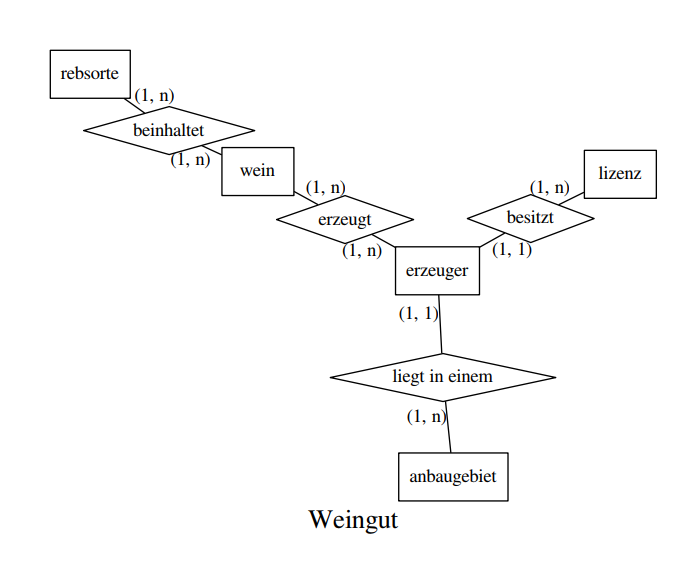
\includegraphics[width=14cm, height=10cm]{images/weingut_neato.png}
		\caption{Weingut Entity-Relationship Diagramm erstellt mittels Graphviz}
		\label{wein}
	\end{center}
\end{figure}
\begin{figure}[H]
	\begin{center}
		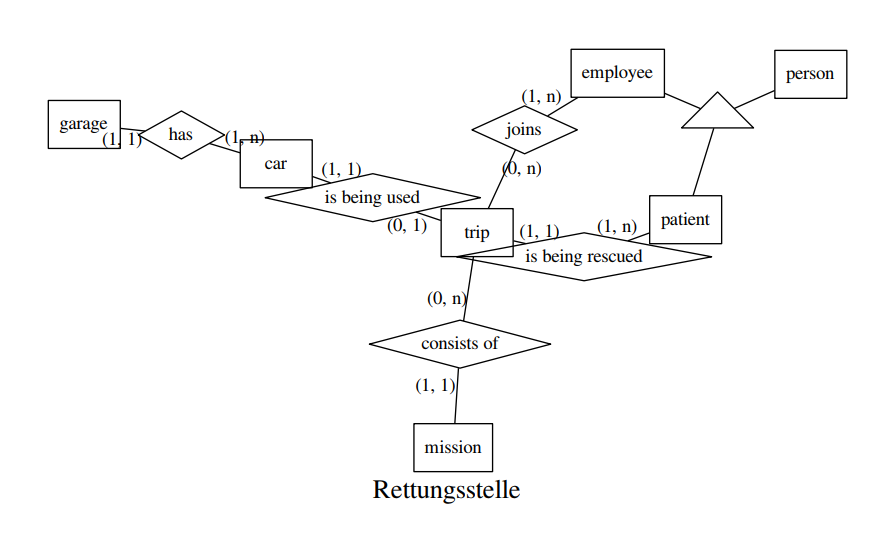
\includegraphics[width=14cm,height=10cm]{images/rettungsstelle_neato.png}
		\caption{Rettungsstelle Entity-Relationship Diagramm erstellt mittels Graphviz}
		\label{rettung}
	\end{center}
\end{figure}

\fib{}
\noindent
An den Abbildung \ref{wein} und Abbildung \ref{rettung} sieht man das sich Graphviz bei kleineren Graphen durchaus geeignet hat.

\begin{figure}[H]
	\begin{center}
		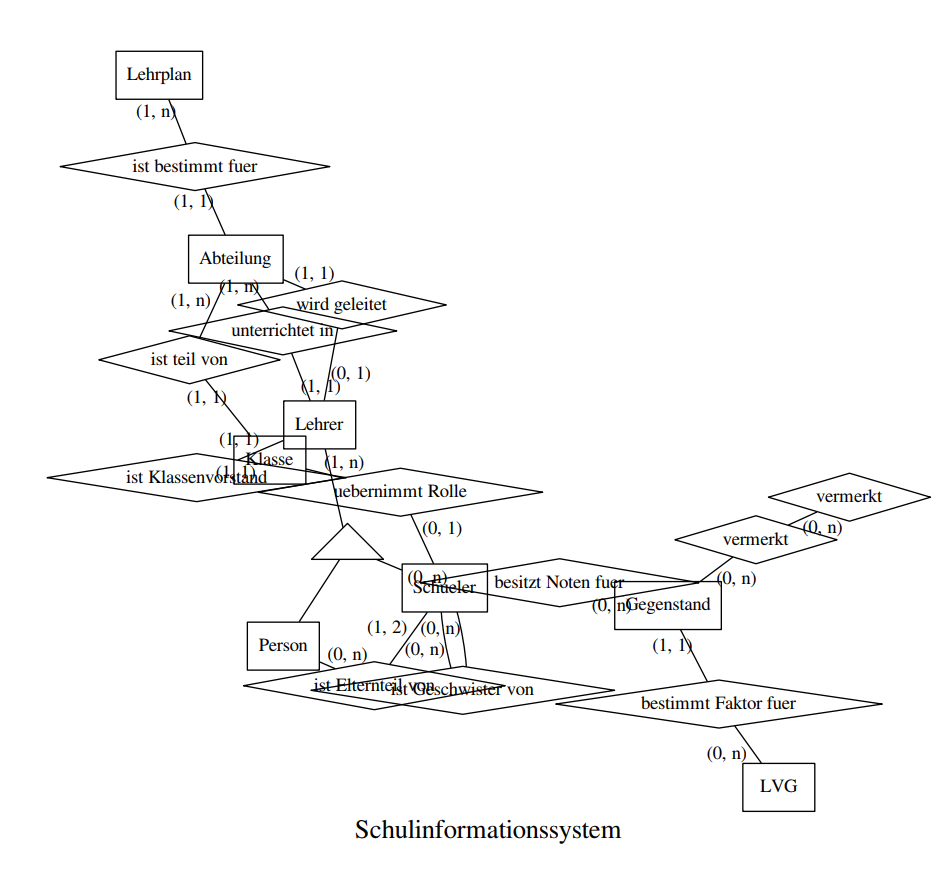
\includegraphics[width=16cm, height=10cm]{images/sis_neato.png}
		\caption{Schulinformationssystem Entity-Relationship Diagramm erstellt mittels Graphviz}
		\label{sis}
	\end{center}
\end{figure}
\noindent
Jedoch sieht man an den Abbildung \ref{sis} das ab einer Gewissen Anzahl an Elementen Graphviz nicht mehr eignet, da es die Elemente wegen Platz mangels, immer enger aneinander positioniert, wodurch der Graph unleserlich wird.